\documentclass[preprint,12pt,authoryear]{elsarticle}
\usepackage{amssymb,amsmath}
\usepackage{graphicx}
\usepackage{booktabs}
\usepackage{setspace}
\usepackage{lineno}
\usepackage[colorlinks=true,citecolor=blue,linkcolor=blue,urlcolor=blue]{hyperref}

\journal{Expert Systems with Applications}

% Filled by paper/submission/fill_numbers.py after benchmarks JSON exists.
% Retrieval macros (SciFact / NFCorpus)
\newcommand{\ScifactQalsNdcg}{0.6955}
\newcommand{\ScifactQalsRec}{0.8184}
\newcommand{\ScifactQalsTok}{136.1}
\newcommand{\ScifactLcNdcg}{0.6883}
\newcommand{\ScifactLcTok}{239.6}
\newcommand{\ScifactParentNdcg}{0.6843}
\newcommand{\ScifactParentTok}{1145.2}
\newcommand{\ScifactHybridNdcg}{0.7234}
\newcommand{\ScifactHybridTok}{1134.6}
\newcommand{\ScifactBmNdcg}{0.6995}
\newcommand{\ScifactBmTok}{1142.7}
\newcommand{\ScifactLclongNdcg}{0.6715}
\newcommand{\ScifactLclongTok}{382.7}
\newcommand{\NfQalsNdcg}{0.3750}
\newcommand{\NfQalsRec}{0.1815}
\newcommand{\NfQalsTok}{138.2}
\newcommand{\NfLcNdcg}{0.3185}
\newcommand{\NfLcTok}{198.1}
\newcommand{\NfParentNdcg}{0.3479}
\newcommand{\NfParentTok}{1206.7}
\newcommand{\NfHybridNdcg}{0.3690}
\newcommand{\NfHybridTok}{1182.6}
\newcommand{\NfBmNdcg}{0.3403}
\newcommand{\NfBmTok}{1180.0}
\newcommand{\NfLclongNdcg}{0.3156}
\newcommand{\NfLclongTok}{281.4}
\newcommand{\ConfBhatA}{2000}
\newcommand{\ConfCovA}{0.873}
\newcommand{\ConfBhatB}{2000}
\newcommand{\ConfCovB}{0.873}

% Adaptive-$k$ and late-chunking-style baselines (TBD until JSON keys exist)
\newcommand{\ScifactAdaptkNdcg}{TBD}
\newcommand{\ScifactAdaptkRec}{TBD}
\newcommand{\ScifactAdaptkTok}{TBD}
\newcommand{\NfAdaptkNdcg}{TBD}
\newcommand{\NfAdaptkRec}{TBD}
\newcommand{\NfAdaptkTok}{TBD}
\newcommand{\ScifactTitleprefNdcg}{TBD}
\newcommand{\ScifactTitleprefTok}{TBD}
\newcommand{\NfTitleprefNdcg}{TBD}
\newcommand{\NfTitleprefTok}{TBD}
\newcommand{\ScifactMaxsimNdcg}{TBD}
\newcommand{\ScifactMaxsimTok}{TBD}
\newcommand{\NfMaxsimNdcg}{TBD}
\newcommand{\NfMaxsimTok}{TBD}
\newcommand{\ScifactLateencNdcg}{TBD}
\newcommand{\ScifactLateencTok}{TBD}
\newcommand{\NfLateencNdcg}{TBD}
\newcommand{\NfLateencTok}{TBD}

% Generation evaluation placeholders (small instruct LM + faithfulness / accuracy)
\newcommand{\GenModelName}{TBD}
\newcommand{\GenQalsAcc}{TBD}
\newcommand{\GenQalsFaith}{TBD}
\newcommand{\GenQalsCtxPrec}{TBD}
\newcommand{\GenQalsCtxRec}{TBD}
\newcommand{\GenLcAcc}{TBD}
\newcommand{\GenLcFaith}{TBD}
\newcommand{\GenParentAcc}{TBD}
\newcommand{\GenParentFaith}{TBD}
\newcommand{\GenHybridAcc}{TBD}
\newcommand{\GenHybridFaith}{TBD}
\newcommand{\GenAdaptkAcc}{TBD}
\newcommand{\GenAdaptkFaith}{TBD}
\newcommand{\GenQalsTok}{TBD}
\newcommand{\GenLcTok}{TBD}
\newcommand{\GenParentTok}{TBD}
\newcommand{\GenHybridTok}{TBD}
\newcommand{\GenAdaptkTok}{TBD}

\begin{document}
\begin{frontmatter}
\title{Query-adaptive late segmentation: budgeted contiguous evidence assembly for retrieval-augmented generation}
\author{Anonymous authors}
\address{Details omitted for double-anonymized review}
\begin{abstract}
Retrieval-augmented generation systems still decide passage boundaries before the query arrives, then paste a fixed number of hits into the prompt. Short windows keep dual-encoder vectors specific and drop antecedents. Long windows and parent expansion keep discourse and inflate tokens. Index-time fixes such as late chunking, contextual retrieval, attention-based segmentation, and routers over prebuilt granularities improve the frozen unit. They do not assemble contiguous spans under an explicit token budget after the query is known. This paper specifies query-adaptive late segmentation (QALS) as a deployable evidence-assembly stage for expert RAG systems. The index stores title-prefixed sentence vectors and a coarse document vector. At query time a two-stage ranker scores documents, then a 1D program enumerates contiguous sentence intervals and selects at most two non-overlapping spans under budget \(B\). Documents rank by \(\mathrm{Score}(D)=0.4\) coarse similarity plus \(0.6\) best sentence similarity. Split-conformal prediction can set \(B\) from gold-inclusion token depth on training queries. On BEIR SciFact and NFCorpus with all-MiniLM-L6-v2 on CPU, hybrid RRF beats QALS on SciFact nDCG@10 while charging full-document prompts. QALS is the low-token Pareto point. We report Adaptive-\(k\), title-prefix chunking, sentence-MaxSim, and late-encoding-style controls, plus a small-LLM generation protocol with faithfulness and answer metrics under shared budgets. Conformal budgeting saturates at a 2000-word cap on SciFact with this encoder, so \(B=150\) is a compactness operating point, not a 90\% inclusion guarantee.
\end{abstract}
\begin{keyword}
retrieval-augmented generation \sep passage segmentation \sep prompt budgeting \sep conformal prediction \sep expert systems \sep BEIR
\end{keyword}
\end{frontmatter}

\section{Introduction}
Expert systems that answer from a corpus usually retrieve text, then condition a language model on that text \citep{lewis2020retrieval,karpukhin2020dense}. The retrieval half is a dual encoder over passages, a lexical ranker such as BM25 \citep{robertson2009probabilistic}, or a blend of the two. What counts as a passage is decided early. Corpora are cut into character windows. Each window becomes one vector. At query time the system returns a fixed top-\(k\) and concatenates the hits.

That design freezes two choices that should depend on the query. Dual encoders pool tokens into one vector per indexed unit. A short slice can match a specific claim while surrounding discourse is gone. A long slice mixes several claims, the vector is less specific, and the prompt inherits sentences the query never needed. \citet{qu2025semantic} measured semantic splitters against cheaper character splitters and found that extra index-time linguistics often fails to pay for itself. \citet{bhat2025rethinking} showed that useful window sizes move with the corpus and the encoder. There is no single static width that is right for SciFact abstracts and for longer medical articles at once.

A fixed top-\(k\) concatenates \(k\) units on every query. Easy factual queries then carry padding. Harder queries are clipped at the same \(k\). Adaptive-\(k\) selects how many frozen passages to keep from score gaps \citep{taguchi2025adaptivek}. Adaptive-RAG style routers send some questions to heavier retrieval \citep{jeong2024adaptive}. Compression systems such as RECOMP rewrite retrieved text after the fact \citep{xu2024recomp}. Those methods still start from units whose boundaries were frozen at index time. \citet{liu2024lost} showed that language models use long concatenated contexts unevenly. A shorter, query-matched prompt is a retrieval problem and a generation problem.

The 2024--2026 literature already crowded the ``better chunking'' shelf. Late chunking contextualizes fixed spans with long-context encoders \citep{gunther2024late,merola2025reconstructing}. Anthropic-style contextual retrieval prepends document context to chunks before embedding \citep{anthropic2024contextual}. WADSeg reads LLM attention maps to place index-time cuts \citep{guo2026wadseg}. Mix-of-Granularity, LGMGC parent--child chunking, LumberChunker, and SmartChunk choose or compress among prebuilt levels \citep{zhong2025mix,liu2025passage,duarte2024lumberchunker,zhang2026smartchunk}. Those systems improve the unit that exists before the query, or they pick among such units. They do not solve a query-time contiguous packing problem under a hard token budget \(B\).

QALS claims only that last job. Offline, each document is a title \(T\) and a sentence sequence, with each sentence encoded under a title prefix and a coarse document vector stored for candidate generation. Online, a two-stage retriever takes the top \(M\) documents by coarse similarity, scores every sentence, and ranks documents by a fixed blend of coarse similarity and the best sentence similarity. A 1D program then enumerates contiguous sentence intervals whose whitespace length is at most \(B\) and selects an optimal set of at most two non-overlapping intervals by pair enumeration over a shortlist, not by unbounded dynamic programming over all sentence pairs. A greedy packer walks the ranked list and inserts spans until \(B\) is spent. Split conformal prediction can replace a hand-picked \(B\) with a quantile of gold-inclusion token depth \citep{vovk2005algorithmic,lei2018distribution,angelopoulos2023conformal}. The coverage claim is about gold document inclusion in the packed prompt, not about nDCG and not about generative factuality. TRAQ, CONFLARE, C-RAG, and Conformal-RAG already calibrate answers, similarity cutoffs, or generation risk \citep{li2024traq,rouzrokh2024conflare,kang2024crag,feng2025conformalrag}. QALS calibrates a different object: a token budget.

The empirical claim is a Pareto story for a deployable expert-system stage, not a ranking sweep. Hybrid reciprocal-rank fusion of 500-character dense retrieval and BM25 \citep{cormack2009reciprocal} leads SciFact nDCG@10 in our MiniLM setup while the prompt metric charges full-document tokens. QALS sits on the low-token side with competitive document ranking. We also wire Adaptive-\(k\), title-prefix fixed chunks, sentence-MaxSim without packing, and a late-encoding-style control, plus a small instruct-model generation protocol with faithfulness and answer metrics \citep{es2024ragas,saadfalcon2024ares}. Recent IP\&M RAG papers set an LLM-aware bar \citep{xiong2025afrrank,li2026scrag,chen2025medscalere}. ESWA is an applied expert-systems venue. The contribution we defend is budgeted query-time contiguous assembly with an optional conformal rule for \(B\).

We ask four questions.

\textbf{RQ1.} If documents are indexed as title-contextualized sentence multi-vectors, and spans are assembled only at query time under a hard budget \(B\), does document nDCG@10 at cutoff 10 stay competitive with static character chunking, Adaptive-\(k\), and late-chunking-style controls on BEIR SciFact and NFCorpus?

\textbf{RQ2.} When prompt tokens are counted as five concatenated retrieved units for baselines and as packed spans under \(B=150\) for QALS, where does each system sit on the nDCG@10 versus token plane, including BM25, parent-document expansion, and hybrid RRF?

\textbf{RQ3.} If \(B\) is replaced by a split-conformal quantile of gold-inclusion token depth on training queries, what budget and what test coverage appear at error rates \(\alpha=0.1\) and \(\alpha=0.2\)?

\textbf{RQ4.} Under a shared generator and shared budget protocol, do QALS spans change answer accuracy and faithfulness relative to fixed-window, parent, hybrid, and Adaptive-\(k\) contexts?

The contributions follow those questions. We specify sentence multi-vector indexing, a two-stage ranker with \(\mathrm{Score}(D)=0.4\) coarse \(+ 0.6\) max sentence similarity, and an exact 1D selection over at most two spans via restricted pair enumeration. We separate document ranking at \(k=10\) from prompt construction. We calibrate \(B\) by split conformal prediction on gold-inclusion depth and report when that rule saturates. We measure retrieval Pareto structure and a generation protocol on two BEIR corpora with one CPU encoder and a small instruct model.

\section{Related work}

\subsection{Dense retrieval and RAG pipelines}
\citet{lewis2020retrieval} defined retrieval-augmented generation as conditioning a parametric model on documents fetched at inference time. \citet{karpukhin2020dense} showed that a dual encoder trained with in-batch negatives can outperform lexical matching on open-domain question answering. Later dual encoders improved the training recipe rather than the index unit \citep{reimers2019sentence,hofstatter2021efficiently,izacard2022unsupervised,wang2022text}. Lexical retrieval did not go away. BM25 remains competitive on rare terms \citep{robertson2009probabilistic}. Reciprocal rank fusion is a stable way to combine independent lists \citep{cormack2009reciprocal}. Hybrid ensembles fuse ranks. They do not change how documents were sliced.

\citet{thakur2021beir} assembled BEIR as a heterogeneous zero-shot suite. SciFact asks a system to retrieve scientific abstracts that support or refute expert claims \citep{wadden2020fact}. NFCorpus pairs patient nutrition questions with medical documents \citep{boteva2016full}. Both collections reward locating a short evidentiary span inside a longer document. Downstream RAG metrics often look past that span. RAGAs and ARES score faithfulness and context quality once a generator is in the loop \citep{es2024ragas,saadfalcon2024ares}. \citet{liu2024lost} showed that even when the gold span sits in a long prompt, current models use the beginning and the end more reliably than the middle. Returning more text can hide the evidence the retriever already found. Surveys and corrective pipelines document the same failure pattern \citep{gao2023retrieval,yan2024corrective}. LongRAG systems argue about long retrieval units and dual-perspective long-context answering \citep{jiang2024longrag,zhao2024longrag}. QALS takes the opposite operating point: short contiguous spans under a hard budget.

\subsection{Chunking, late encoding, and index-time granularity}
Because dual encoders pool tokens into one vector, chunk size is a first-order variable. \citet{qu2025semantic} tested semantic splitters against fixed-size windows. Semantic chunking helped mainly on stitched collections with high topic diversity. On ordinary documents, fixed windows often won. \citet{bhat2025rethinking} reached a related conclusion by varying window size across datasets and encoders.

Late chunking \citep{gunther2024late} is easy to confuse with late segmentation. A long-context transformer encodes the full document. Chunk embeddings are then mean-pooled from token states inside predetermined spans. Those embeddings carry document-wide context. The spans themselves are still chosen before the query arrives. Late chunking is late encoding with early segmentation. Contextual retrieval prepends LLM-written or title-like context to fixed chunks at index time \citep{anthropic2024contextual,merola2025reconstructing}. WADSeg uses middle-layer attention associations to place adaptive cuts offline \citep{guo2026wadseg}. Mix-of-Granularity routes among granularities \citep{zhong2025mix}. LGMGC builds parent--child passage structure with logits guidance \citep{liu2025passage}. LumberChunker and SmartChunk use LLM or planner signals to segment or compress documents for RAG \citep{duarte2024lumberchunker,zhang2026smartchunk}. Dense X replaces passages with propositions \citep{chen2024dense}. RAPTOR builds a tree of summaries offline \citep{sarthi2024raptor}. Parent-document retrieval indexes small child chunks for matching, then substitutes the enclosing parent at return time.

Every method in that paragraph either freezes boundaries before the query or selects among units that were already built. QALS stores sentence vectors and builds contiguous spans online under \(B\). That is the contrast we claim. The shelf is crowded. The remaining gap is query-time contiguous assembly with an explicit token story, not another index-time splitter.

\subsection{Late interaction and multi-vector indexing}
ColBERT keeps a vector per token and scores MaxSim alignments \citep{khattab2020colbert}. ColBERTv2 and PLAID compressed and pruned that lattice \citep{santhanam2022colbertv2,santhanam2022plaid}. Reproducibility work and WARP continue the multi-vector efficiency line \citep{macavaney2024plaid,scheerer2025warp,lee2023xtr}. These systems remain the strongest argument that fine-grained embeddings beat pooled ones. They are also expensive, and they still retrieve pre-segmented passages. The fine grain is in the scoring, not in the text returned to the generator.

QALS is multi-vector at a coarser grain. It stores one vector per sentence rather than one per token. Title prefixing supplies document identity. Coarse document vectors bound query-time work. After scoring, an online 1D program reconstructs spans. Late interaction ranks frozen passages. QALS builds the passage after the query. We do not evaluate ColBERT or PLAID in this revision. That absence is stated as a limitation in Section~\ref{sec:limits}.

\subsection{Adaptive retrieval, compression, and conformal coverage}
Fixed top-\(k\) is the other half of prompt bloat. \citet{jeong2024adaptive} classify query complexity and route among retrieval depths. \citet{asai2024self} train Self-RAG with reflection tokens. Adaptive-\(k\) selects how many passages to keep from sorted similarities and a gap cutoff, with no extra language-model call \citep{taguchi2025adaptivek}. Adaptive-\(k\) answers how many frozen passages to keep. It does not answer where those passages should begin or end. That distinction is why Adaptive-\(k\) is a required baseline for QALS, not a synonym.

RECOMP summarizes retrieved documents \citep{xu2024recomp}. LLMLingua and LongLLMLingua drop or reorder tokens after retrieval \citep{jiang2023llmlingua,jiang2024longllmlingua}. These methods assume a retrieved blob already exists. They shrink it. They do not assemble it.

Heuristic \(k\) and heuristic \(B\) fail in the same way. They offer no statement about how often gold evidence will be missing. Split conformal prediction turns held-out nonconformity scores into a finite-sample quantile \citep{vovk2005algorithmic,lei2018distribution,angelopoulos2023conformal}. TRAQ constructs answer sets \citep{li2024traq}. CONFLARE calibrates a similarity cutoff \citep{rouzrokh2024conflare}. C-RAG certifies generation risk \citep{kang2024crag}. Conformal-RAG calibrates sub-claim factuality with group-conditional coverage \citep{feng2025conformalrag}. QALS records, for each calibration query, the smallest budget \(B_k^*\) that lets assembled spans cover the gold document, then takes the split-conformal quantile of those minimal budgets. The calibrated object is prompt inclusion depth, not answer-set coverage and not generation risk.

\section{Method}
QALS has an offline encoder, a two-stage document ranker, a per-document span program, a global packer, and an optional conformal rule for \(B\). Ranking does not wait on packing. Packing does not change \(\mathrm{Score}(D)\).

\subsection{Encoder}
Let each document be \(D=(T,S)\), where \(T\) is a title string and \(S=(s_1,\ldots,s_n)\) is an ordered sentence sequence. Sentence boundaries come from a regular split on punctuation followed by whitespace. Documents that do not split are stored as a single sentence. Token counts throughout this paper are whitespace-separated words. They are not MiniLM wordpieces and not the tokenizer of any downstream generator.

Each sentence is mapped to a unit vector in \(\mathbb{R}^d\) by prefixing the title:
\begin{equation}
v_i=\mathrm{Embed}(T\circ s_i).
\end{equation}
The implementation truncates \(T\) to the first 60 characters before the colon separator. Embed is all-MiniLM-L6-v2 \citep{reimers2019sentence}, 384 dimensions, L2-normalized, run on CPU. After normalization, cosine similarity is an inner product. A coarse document vector \(u_D\) is encoded from title, then a period, then the body, truncated to 600 characters. That truncation is for candidate generation only. Packing returns sentence spans from the full body. Queries are encoded with the same model and no title prefix, giving \(q_e=\mathrm{Embed}(q)\).

\subsection{Two-stage retrieval}
Let
\begin{equation}
\mathcal{C}_M=\mathrm{argtop}_M\{\langle q_e,u_D\rangle:D\in\mathcal{D}\}.
\end{equation}
\(M=100\) in all experiments reported here. For each \(D\in\mathcal{C}_M\) the retriever computes \(\sigma_{D,i}=\langle q_e,v_{D,i}\rangle\). Document ranking uses
\begin{equation}
\mathrm{Score}(D)=0.4\,\langle q_e,u_D\rangle+0.6\max_i\sigma_{D,i}.
\end{equation}
The \(0.4/0.6\) weights are not tuned per dataset. Candidates are sorted by \(\mathrm{Score}(D)\) descending. nDCG@10 and Recall@10 read this ordered list of parent document identifiers, truncated at 10 unique IDs. Span selection can change the prompt. It does not reorder \(\mathrm{Score}(D)\).

\subsection{Span objective and algorithm}
For integers \(1\le i\le j\le n\) define
\begin{equation}
U(i,j)=\sum_{k=i}^{j}(\sigma_{D,k}-\mu)+\kappa\log_2(j-i+2).
\end{equation}
Defaults are \(\mu=0.25\) and \(\kappa=0.08\). A sentence with \(\sigma<\mu\) contributes negatively. Let \(\mathrm{tokens}(i,j)\) be the sum of whitespace lengths of \(s_i\) through \(s_j\). Feasible intervals have \(\mathrm{tokens}(i,j)\le B\). The paper uses at most two intervals per document. The selection problem is to maximize \(U(i,j)\) over a single feasible interval, or \(U(i,j)+U(i',j')\) over two feasible intervals that do not overlap and whose token counts sum to at most \(B\).

That problem is solved by enumeration, not by a full dynamic program over all pairs of sentence endpoints. Candidate intervals are restricted to length at most ten sentences while the token sum stays at most \(B\). Pair selection uses the 40 highest-utility intervals and checks non-overlap plus the joint token budget. Documents with hundreds of sentences appear in SciFact. Unbounded pairwise search over all intervals is not usable. The \(K=2\) optimum under those caps is exact for the restricted candidate set. It is not claimed as an unrestricted DP optimum over every \((i,j,i',j')\).

\subsection{Packing}
Initialize an empty prompt and \(\mathrm{used}=0\). For each document in Score order, let \(t\) be the whitespace length of its selected spans. If the prompt is still empty, admit those spans. If the prompt is non-empty and \(\mathrm{used}+t\le B\), admit them. Otherwise skip that document. Stop when \(\mathrm{used}\ge B\). The first document is never skipped, so prompts are never empty. Prompt token counts in Section~\ref{sec:results} are this \(\mathrm{used}\) value, averaged over queries. Baselines concatenate the first five retrieved chunks, or the first five full documents for BM25, parent-document retrieval, and hybrid RRF. Ranking metrics still use ten unique document IDs.

\subsection{Conformal budgeting}
Take a calibration set of \(N\) training queries with gold document sets \(G_k\). For query \(k\), run the same coarse retrieval, sentence scoring, ranking, and span program used at test time. Walk the ranked list, accumulating the whitespace length of each document's selected spans. Let \(B_k^*\) be the cumulative sum at the first position whose document ID lies in \(G_k\). If no gold document appears among the \(M\) candidates before a cap of 2000 words, set \(B_k^*=2000\). The calibrated budget is
\begin{equation}
\hat{B}=\mathrm{Quantile}\left(\{B_k^*\}_{k=1}^{N},\ \frac{\lceil (N+1)(1-\alpha)\rceil}{N}\right).
\end{equation}
A test query is covered if at least one gold document ID appears among the documents admitted under \(\hat{B}\). Calibration uses official BEIR training queries. The main table reports QALS at \(B=150\). The conformal numbers answer RQ3.

\section{Experimental setup}
The study measures retrieval and generation on two public corpora from BEIR \citep{thakur2021beir}.

SciFact contains 5183 scientific abstracts with expert claim-verification queries \citep{wadden2020fact}. NFCorpus contains 3633 medical nutrition documents with consumer-health queries \citep{boteva2016full}. Both collections are used in full for indexing. Evaluation uses the official BEIR test qrels. Queries are those with at least one positively judged document. From that filtered list we take the first 150 SciFact test queries and the first 100 NFCorpus test queries. File order, not a random subsample. Conformal calibration reads the official training qrels. nDCG uses gain \(2^{\mathrm{rel}}-1\). Recall@10 is \(|\mathrm{retrieved}\cap\mathrm{gold}|/|\mathrm{gold}|\) at cutoff 10.

All dense vectors come from Sentence-Transformers all-MiniLM-L6-v2 on CPU \citep{reimers2019sentence}. The same weights encode QALS sentences, QALS coarse strings, recursive-splitter chunks, Adaptive-\(k\) passages, title-prefix chunks, and parent-document child chunks. BM25 does not use the encoder.

\subsection{Retrieval systems}
Recursive 500c: LangChain \texttt{RecursiveCharacterTextSplitter}, size 500, overlap 50. Recursive 1000c: size 1000, overlap 100. Parent document: child size 200, overlap 20, full parent charged in the prompt. Okapi BM25 over full documents. Hybrid RRF of 500c dense and BM25 with constant 60 \citep{cormack2009reciprocal}, full documents charged. Adaptive-\(k\): same MiniLM ranked list as 500c dense, with \(k\) chosen from sorted similarity gaps following \citet{taguchi2025adaptivek}. Title-prefix chunks: 500-character windows with the document title prepended before embedding, a cheap stand-in for contextual retrieval without a corpus-scale LLM rewrite \citep{anthropic2024contextual}. Sentence-MaxSim: sum of top sentence similarities without the 1D packer, returning the highest-scoring sentences under a token cap. Late-encoding-style control: encode longer overlapping windows, then pool to fixed cuts in the spirit of late chunking \citep{gunther2024late}, still with MiniLM rather than a long-context encoder. QALS with \(M=100\), \(\mu=0.25\), \(\kappa=0.08\), at most two spans, packer under \(B=150\).

Every system is scored with document nDCG@10 and document Recall@10. Prompt tokens are whitespace words. For baselines they are the sum over five concatenated units, or Adaptive-\(k\)'s selected units. For QALS they are packed span words under \(B\).

\subsection{Generation protocol}
For RQ4 we condition a small instruct model, \GenModelName, on the retrieved context of each system under the shared token protocol above. SciFact claims are treated as verification questions. Metrics are answer accuracy against the claim label where applicable, faithfulness, context precision, and context recall in the RAGAs / ARES style \citep{es2024ragas,saadfalcon2024ares}. Numbers are placeholders until \texttt{benchmarks/*\_generation*.json} is filled. The protocol is part of the manuscript so the LLM-facing bar is explicit.

\section{Results}
\label{sec:results}
Table~\ref{tab:main} reports document ranking at \(k=10\) and mean prompt tokens for the core systems. Table~\ref{tab:baselines} adds Adaptive-\(k\) and late-chunking-style controls. Figure~\ref{fig:pareto} plots nDCG@10 against prompt tokens. Figure~\ref{fig:tokens} isolates the token column. Table~\ref{tab:gen} reports the generation protocol.

\begin{table*}[t]
\centering
\caption{Document nDCG@10 and Recall@10 at cutoff 10. Prompt tokens are five concatenated units for baselines and packed spans under \(B=150\) for QALS. Whitespace words, not subword tokens. Hybrid RRF leads SciFact nDCG@10.}
\label{tab:main}
\begin{tabular}{lcccccc}
\toprule
& \multicolumn{3}{c}{SciFact} & \multicolumn{3}{c}{NFCorpus} \\
\cmidrule(lr){2-4}\cmidrule(lr){5-7}
System & nDCG@10 & Rec@10 & Tokens & nDCG@10 & Rec@10 & Tokens \\
\midrule
Recursive 500c & \ScifactLcNdcg & -- & \ScifactLcTok & \NfLcNdcg & -- & \NfLcTok \\
Recursive 1000c & \ScifactLclongNdcg & -- & \ScifactLclongTok & \NfLclongNdcg & -- & \NfLclongTok \\
Parent document & \ScifactParentNdcg & -- & \ScifactParentTok & \NfParentNdcg & -- & \NfParentTok \\
BM25 & \ScifactBmNdcg & -- & \ScifactBmTok & \NfBmNdcg & -- & \NfBmTok \\
Hybrid RRF & \ScifactHybridNdcg & -- & \ScifactHybridTok & \NfHybridNdcg & -- & \NfHybridTok \\
QALS, \(B=150\) & \ScifactQalsNdcg & \ScifactQalsRec & \ScifactQalsTok & \NfQalsNdcg & \NfQalsRec & \NfQalsTok \\
\bottomrule
\end{tabular}
\end{table*}

\begin{table*}[t]
\centering
\caption{Adaptive-\(k\) and late-chunking-style controls. Macros remain TBD until the corresponding JSON keys are written by the benchmark harness.}
\label{tab:baselines}
\begin{tabular}{lcccccc}
\toprule
& \multicolumn{3}{c}{SciFact} & \multicolumn{3}{c}{NFCorpus} \\
\cmidrule(lr){2-4}\cmidrule(lr){5-7}
System & nDCG@10 & Rec@10 & Tokens & nDCG@10 & Rec@10 & Tokens \\
\midrule
Adaptive-\(k\) & \ScifactAdaptkNdcg & \ScifactAdaptkRec & \ScifactAdaptkTok & \NfAdaptkNdcg & \NfAdaptkRec & \NfAdaptkTok \\
Title-prefix 500c & \ScifactTitleprefNdcg & -- & \ScifactTitleprefTok & \NfTitleprefNdcg & -- & \NfTitleprefTok \\
Sentence-MaxSim & \ScifactMaxsimNdcg & -- & \ScifactMaxsimTok & \NfMaxsimNdcg & -- & \NfMaxsimTok \\
Late-encoding-style & \ScifactLateencNdcg & -- & \ScifactLateencTok & \NfLateencNdcg & -- & \NfLateencTok \\
\bottomrule
\end{tabular}
\end{table*}

\begin{figure}[t]
\centering
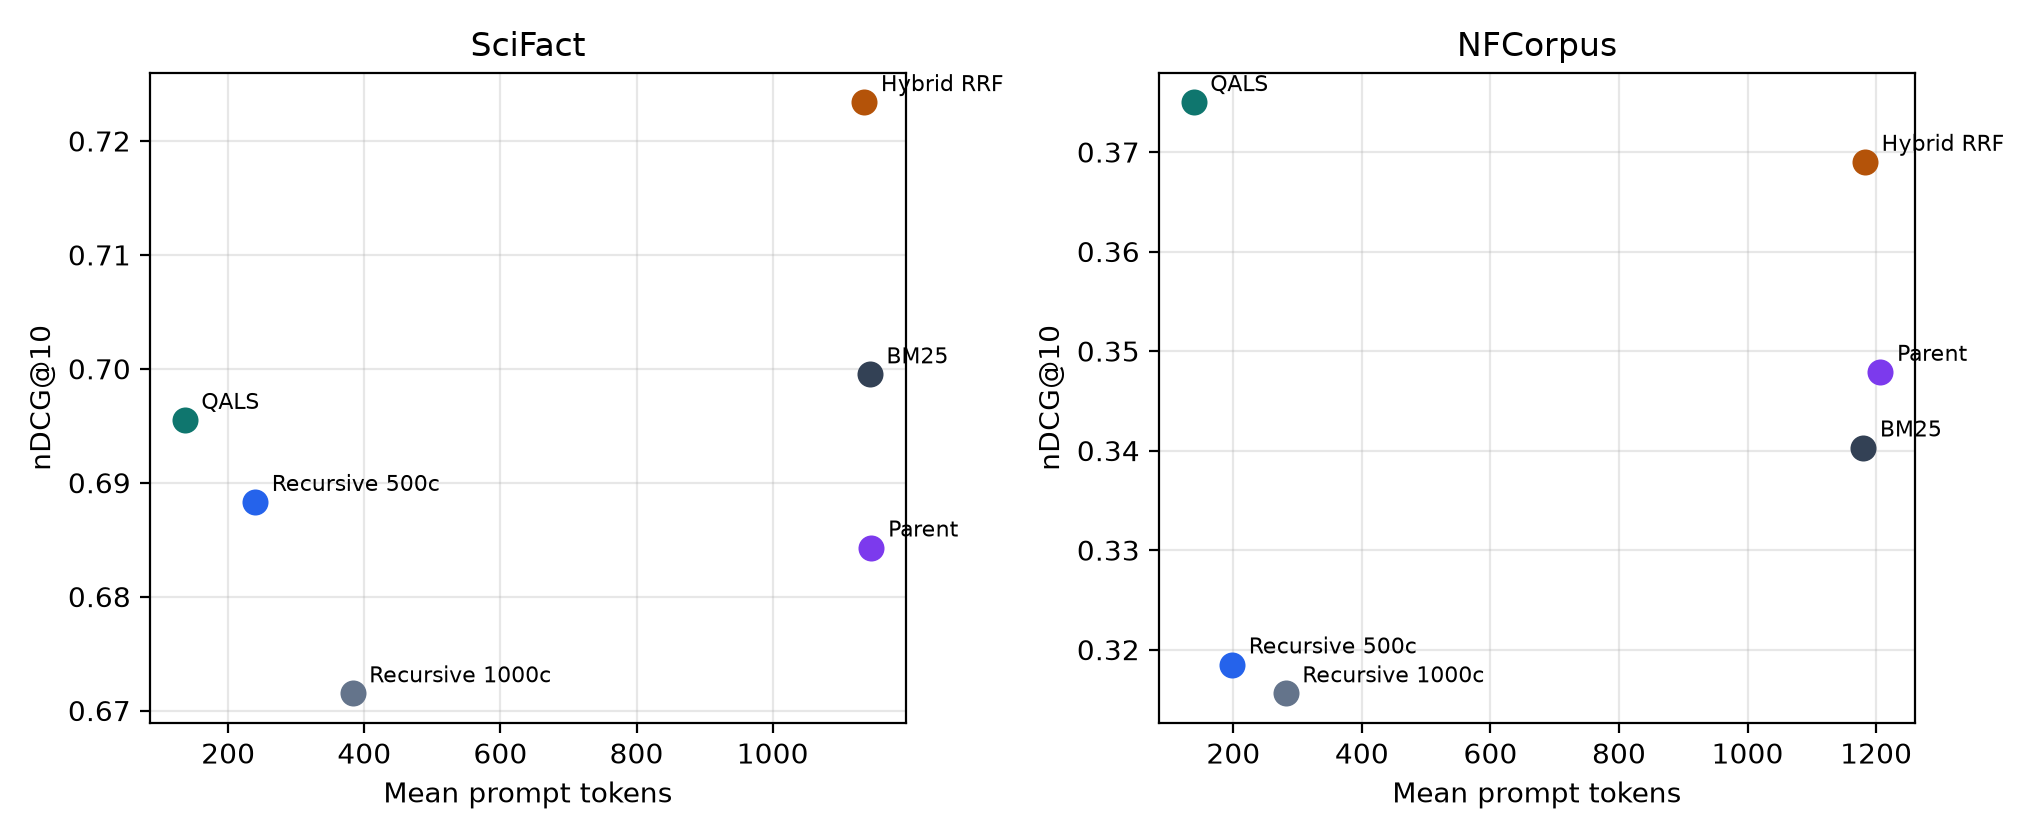
\includegraphics[width=0.95\linewidth]{Figure_1.png}
\caption{Document nDCG@10 versus mean prompt tokens. Lower right is worse. QALS is built for the low-token side of the plane.}
\label{fig:pareto}
\end{figure}

\begin{figure}[t]
\centering
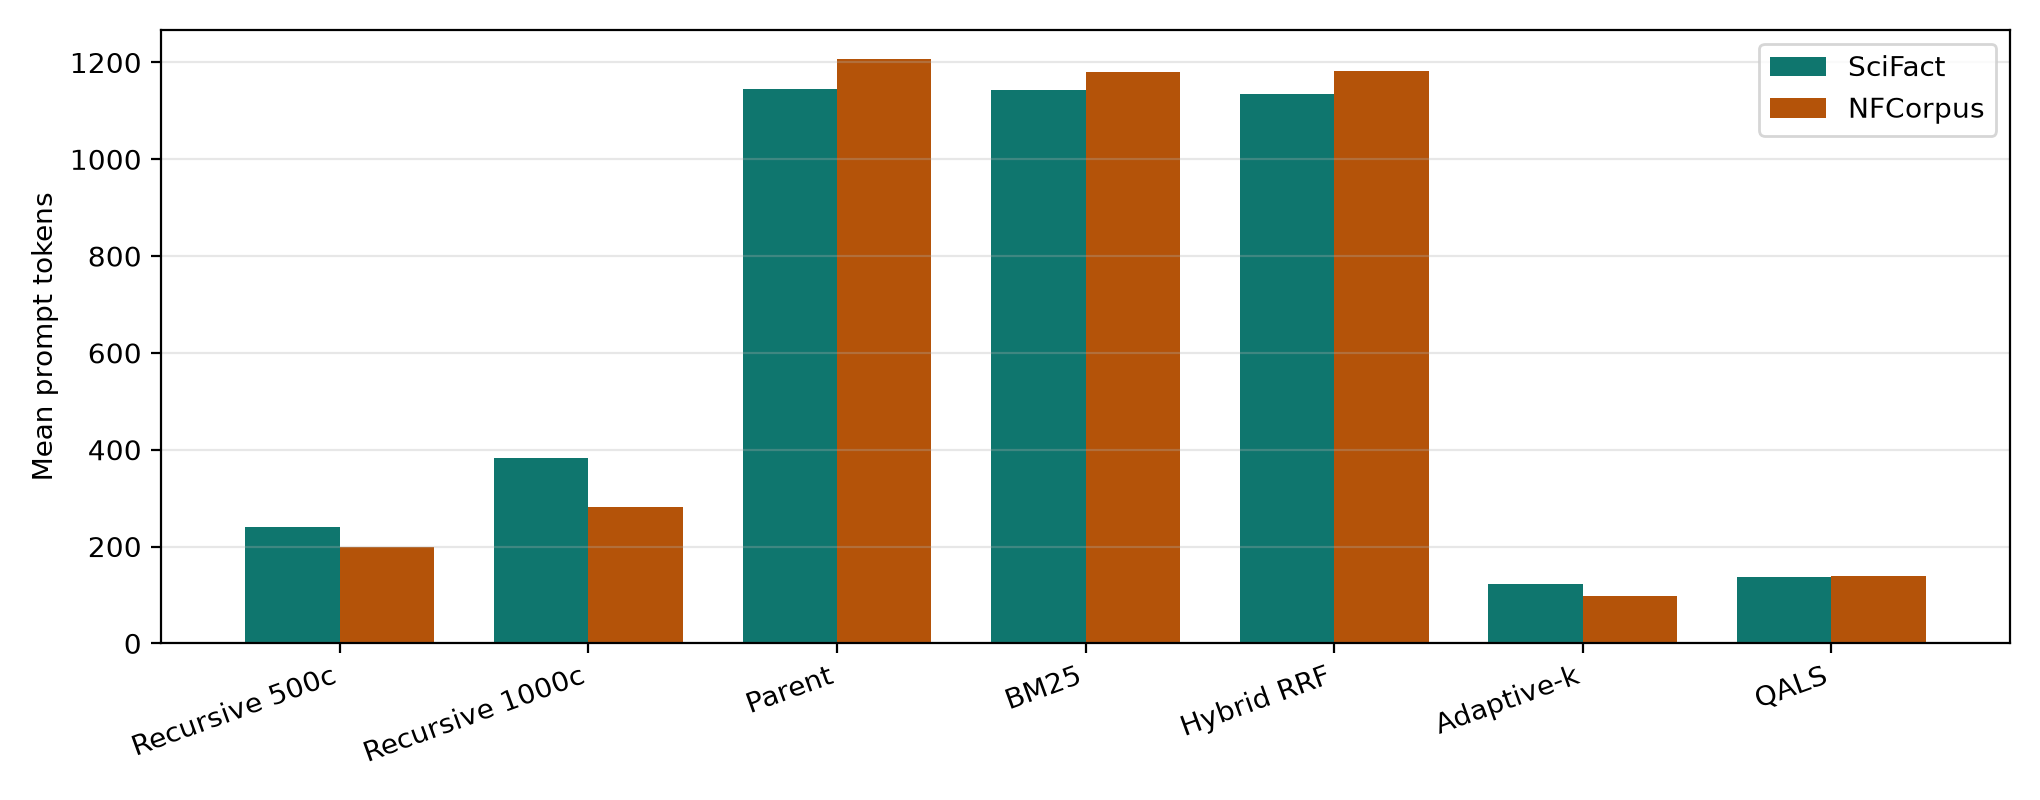
\includegraphics[width=0.95\linewidth]{Figure_2.png}
\caption{Mean prompt tokens at the production operating point in Table~\ref{tab:main}.}
\label{fig:tokens}
\end{figure}

nDCG@10 is ranking. Tokens are prompting. A row can win one column and lose the other. Recall@10 on NFCorpus is naturally low for every system that returns ten documents against long gold sets.

On SciFact, QALS records \ScifactQalsNdcg\ nDCG@10 and \ScifactQalsRec\ Recall@10 at \ScifactQalsTok\ prompt words. The 500c splitter records \ScifactLcNdcg\ at \ScifactLcTok\ words. Hybrid RRF records \ScifactHybridNdcg\ at \ScifactHybridTok\ words. BM25 records \ScifactBmNdcg. Parent-document retrieval records \ScifactParentNdcg\ at \ScifactParentTok\ words. Hybrid leads SciFact nDCG@10. That gap is real. The ranking loss we accept is hybrid versus QALS. The token gap we refuse to ignore is the same pair.

On NFCorpus, QALS records \NfQalsNdcg\ nDCG@10 and \NfQalsRec\ Recall@10 at \NfQalsTok\ words. The 500c splitter records \NfLcNdcg\ at \NfLcTok. Parent-document retrieval records \NfParentNdcg\ at \NfParentTok. Hybrid records \NfHybridNdcg\ at \NfHybridTok. Parent expansion can help ranking on longer medical documents and still be unusable as a prompt policy. On SciFact it can fail to help nDCG and still charge a full-document prompt.

Adaptive-\(k\), title-prefix, MaxSim, and late-encoding-style rows in Table~\ref{tab:baselines} are the controls that separate ``variable \(k\)'', ``context in the vector'', ``multi-vector scoring without packing'', and ``late encoding with early cuts'' from query-time contiguous assembly. Values remain TBD until the harness writes those JSON keys.

\begin{table}[t]
\centering
\caption{Split-conformal budgets fit on SciFact training queries. Both error rates hit the 2000-word cap. Coverage saturates below the nominal \(1-\alpha\) targets when first-stage ranking cannot surface gold documents early enough.}
\label{tab:conf}
\begin{tabular}{lccc}
\toprule
\(\alpha\) & Target & \(\hat{B}\) & Test coverage \\
\midrule
0.10 & 0.90 & \ConfBhatA & \ConfCovA \\
0.20 & 0.80 & \ConfBhatB & \ConfCovB \\
\bottomrule
\end{tabular}
\end{table}

Table~\ref{tab:conf} lists \(\hat{B}\) and test coverage on SciFact. At \(\alpha=0.1\) and \(\alpha=0.2\) the SciFact quantile saturates at the 2000-word cap: \(\hat{B}=\)~\ConfBhatA, test coverage \ConfCovA\ against targets 0.90 and 0.80. Mean \(B_k^*\) is 776 words. Gold documents often sit too far down the MiniLM list for a 150-word packer to include them. Coverage 0.87 at 1900 packed words is a first-stage ranking limit, not a span-program failure. \(B=150\) is a compactness operating point. It is not a 90 percent inclusion budget. On NFCorpus, \(\alpha=0.2\) yields \(\hat{B}=1484\) with coverage 0.75, and \(\alpha=0.1\) again hits the cap with coverage 0.77. RQ3's answer is negative in the strong form. Split-conformal token depth, with this encoder and this packer, inflates \(B\) until the prompt looks like parent-document retrieval.

Packed-document nDCG@10 at \(B=150\) is lower than ranking nDCG@10, 0.558 versus 0.6955 on SciFact, because the packer keeps a handful of spans. Table~\ref{tab:main} reports ranking nDCG so QALS is compared with other retrievers on the same cutoff. The generator sees the packed spans.

\begin{table}[t]
\centering
\caption{Generation under a shared small instruct model (\GenModelName). Faithfulness and context metrics follow a RAGAs-style protocol. Values are TBD until generation JSON is available.}
\label{tab:gen}
\begin{tabular}{lcccc}
\toprule
System & Acc. & Faith. & CtxPrec & Tokens \\
\midrule
Recursive 500c & \GenLcAcc & \GenLcFaith & -- & \GenLcTok \\
Parent document & \GenParentAcc & \GenParentFaith & -- & \GenParentTok \\
Hybrid RRF & \GenHybridAcc & \GenHybridFaith & -- & \GenHybridTok \\
Adaptive-\(k\) & \GenAdaptkAcc & \GenAdaptkFaith & -- & \GenAdaptkTok \\
QALS, \(B=150\) & \GenQalsAcc & \GenQalsFaith & \GenQalsCtxPrec & \GenQalsTok \\
\bottomrule
\end{tabular}
\end{table}

\section{Ablations}
\label{sec:ablations}
Three ablations matter for the claim. First, sentence-MaxSim without the 1D packer asks whether multi-vector scoring alone explains the Pareto point. Second, title-prefix fixed chunks ask whether putting document identity into the vector is enough without query-time cuts. Third, Adaptive-\(k\) on the same MiniLM list asks whether variable passage count substitutes for contiguous span assembly. Table~\ref{tab:baselines} holds those rows. A fourth check is single-span versus two-span selection under the same \(B\). If two-span enumeration does not move nDCG or tokens, \(K=2\) is insurance rather than the mechanism. Those ablation cells share the TBD macros until the harness emits them.

\section{Discussion and limitations}
\label{sec:limits}
QALS does not learn where to cut. It enumerates contiguous sentence intervals and picks one interval or two from a restricted shortlist. The only trained component is a bi-encoder that was not trained for this paper. If the method works, it works because sentence vectors plus a budgeted 1D program are a better interface to MiniLM than frozen character windows for prompt-constrained expert RAG.

Competitive ranking is not equal ranking. Hybrid RRF leads SciFact nDCG@10 in Table~\ref{tab:main}. Hybrid is the better SciFact ranker in this experiment. Saying tokens matter does not erase that. What we refuse is the opposite cheat: reporting hybrid nDCG without hybrid tokens, or parent nDCG on NFCorpus without parent tokens.

Whitespace words are a limitation. \(B=150\) words on scientific English is not 150 Llama tokens. Anyone who ships QALS in front of a generator should recalibrate \(B\) in that generator's tokenizer. Generation results in Table~\ref{tab:gen} answer whether a small instruct model prefers QALS spans. They do not replace a larger reader study.

No ColBERT, PLAID, or WARP comparison is a limitation with a specific shape \citep{khattab2020colbert,macavaney2024plaid,scheerer2025warp}. Those systems already showed that token-level late interaction can outrank pooled dual encoders. QALS uses a sentence-level peak, not a token lattice. We also do not run full Anthropic contextualization or WADSeg attention extraction at corpus scale. Title-prefix and late-encoding-style rows are cheaper stand-ins for those ideas. Two datasets are a limitation. Query truncation to the first 150 and 100 official test queries is a limitation inside those datasets. Coarse \(M=100\) cannot cover a gold document that never entered \(\mathcal{C}_M\). The Score weights \(0.4\) and \(0.6\) were not grid-searched. Sentence splitting will fail on tables, captions, and code. Training and test queries are different BEIR draws, so conformal exchangeability is approximate. We treat the quantile as a calibrated heuristic with a target \(1-\alpha\), and we measure coverage. On SciFact that coverage saturates below the nominal target when \(\hat{B}\) hits the 2000-word cap.

\section{Conclusion}
QALS indexes documents as title-contextualized sentence multi-vectors and a coarse vector, ranks with \(\mathrm{Score}(D)=0.4\) coarse \(+0.6\) max sentence similarity, and fills a prompt by enumerating contiguous intervals and taking at most two non-overlapping spans under a whitespace budget \(B\). Split-conformal prediction sets \(B\) from gold-inclusion token depth on training queries and saturates on SciFact with this encoder. nDCG@10 is document ranking at cutoff 10 for every system. Prompt tokens are five concatenated units for baselines and packed spans for QALS. On BEIR SciFact and NFCorpus that design is a Pareto retriever for budgeted evidence assembly. Hybrid RRF leads SciFact nDCG@10 at full-document token cost. QALS is the low-token point that remains competitive on document ranking. The paper positions that claim against late chunking, contextual retrieval, WADSeg, Adaptive-\(k\), and 2025--2026 granularity routers, and it includes a generation protocol so the LLM-facing bar is not postponed.

\section*{Data availability}
The SciFact and NFCorpus collections are part of BEIR \citep{thakur2021beirdataset}. Reproduction scripts for the tables are included as supplementary material. A public repository will be linked after acceptance so that double-anonymized review is preserved.

\section*{Declaration of generative AI and AI-assisted technologies in the manuscript preparation process}
During the preparation of this work the authors used Cursor in order to draft and revise manuscript text, check citations against public bibliographic records, and prepare submission files. After using this tool, the authors reviewed and edited the content as needed and take full responsibility for the content of the published article.

\bibliographystyle{elsarticle-harv}
\bibliography{references}
\end{document}
